\documentclass[12pt]{article}

\usepackage{arxiv}

\usepackage[utf8]{inputenc} % allow utf-8 input
\usepackage[T1]{fontenc}    % use 8-bit T1 fonts
\usepackage{hyperref}       % hyperlinks
\usepackage{url}            % simple URL typesetting
\usepackage{booktabs}       % professional-quality tables
\usepackage{amsfonts}       % blackboard math symbols
\usepackage{nicefrac}       % compact symbols for 1/2, etc.
\usepackage{microtype}      % microtypography
\usepackage{lipsum}
\usepackage{amsmath}
\usepackage{CJKutf8}
\usepackage{graphics}
\usepackage{abstract}


\title{深度卷积神经网络对\textsf{Imagenet}的分类}

\author{
  Alex Krizhevsky \\
  多伦多大学\\
  \texttt{kriz@cs.utoronto.ca} \\
  %% examples of more authors
   \And
 Ilya Sutskever \\
  多伦多大学\\
  \texttt{ilya@cs.utoronto.ca} \\
  %% examples of more authors
  \And
 Geoffrey E. Hinton\\
  多伦多大学\\
  \texttt{hinton@cs.utoronto.ca}
}  
  %% \AND
  %% Coauthor \\
  %% Affiliation \\
  %% Address \\
  %% \texttt{email} \\
  %% \And
  %% Coauthor \\
  %% Affiliation \\
  %% Address \\
  %% \texttt{email} \\
  %% \And
  %% Coauthor \\
  %% Affiliation \\
  %% Address \\
  %% \texttt{email} \\

\date{}
\renewcommand{\figurename}{图}
\renewcommand{\tablename}{表格}
\begin{document}
\begin{CJK*}{UTF8}{gkai}\CJKindent
\maketitle

\renewcommand{\abstractname}{\Large摘要}
\begin{abstract}

我们训练了一个大规模的深度卷积神经网络,将ImageNet LSVRC-2010比赛中的120万个高分辨率图像分为1000种不同类别。在测试数据上,我们得到的top-1和top-5的误差率分别为37.5\%和17.0\%,这个结果远远优于当前的最佳水平。这个神经网络包含6千万个参数和65万个神经元,还包含了5个卷积层(某些卷积层的后面有最大池化层)以及3个全连接层,最后一个层是1000维的softmax。为了加快训练速度,我们使用了非饱和神经元以及一种基于GPU的高效的卷积运算方法。为了减少全连接层的过拟合,我们运用了最新的正则化方法“dropout”,结果证明它是非常有效的。我们也使用这个模型的变种参加了ILSVRC-2012比赛,相比第二名在top-5上26.2\%的误差率,我们以15.3\%的误差率取胜。
\end{abstract}


% keywords can be removed
%\keywords{First keyword \and Second keyword \and More}


\section{介绍}
\setlength{\parindent}{2em}当前的目标识别方法基本上都使用了机器学习的方法。为了提高这些方法的性能,我们可以收集更多的数据,学习得到更加强大的模型,用更好的方法来防止过拟合。直到现在,有标签的数据集都是比较小的,一般只有万张的数量级(如NORB[16],Caltech-101/256[8,9],以及CIFAR-10/100[12])。在这个大小的数据集上,可以很好的解决简单的识别任务,尤其是在通过标签保留变换进行数据增强的情况下。例如,目前在MNIST数据集上面数字识别最小的误差率(<0.3\%)已经接近了人类的水平[4]。但是现实世界中的目标呈现出很大的可变性,所以要去学习识别他们就需要使用更大的训练数据集。实际上,人们也已广泛地认识到小的图像数据集的缺点(如Pinto等[21]),但直到最近,才能够收集到包含数百万图像的带标签数据集。这些新的大型数据集包括LabelMe[23](包含数十万张被完全分割的图片),ImageNet[6](由1500万张被标记的高清图片组成,覆盖了2.2万个类别)\\

\setlength{\parindent}{2em}为了从数百万张图片中学习到数千种目标,我们需要一个学习能力极强的模型。然而,物体识别任务极高的复杂度意味着即使拥有ImageNet这么大的数据集,这个问题也很难被具体化。所以我们也需要大量关于模型的先验知识去弥补我们缺失的数据。卷积神经网络(CNNs)是一种这样的模型[16,11,13,18,15,22,26]。他们的学习能力可以通过控制网络的深度和宽度来调整,他们也可以对图像的本质做出强大且基本准确的假设(也就是说,统计上的稳定性,以及像素依赖的局部性)。因此,与相似大小的标准前馈神经网络相比,CNNs的连接和参数更少,所以更易训练,而他们理论上的最佳性能仅比标准前馈神经网络稍差一点。\\

\setlength{\parindent}{2em}尽管CNNs有很好的质量,和更有效率的局部结构,但将他们大规模的应用到高分辨率的图像中仍然需要付出高昂的代价。幸运的是,当前的GPU搭配上高度优化的2D卷积实现,已经足够强大到去加速大型CNNs的训练过程,并且最近的数据集例如ImageNet已经包含足够的有标签样本,能够训练出不会严重过拟合的模型。\\

\setlength{\parindent}{2em}本文的具体贡献如下:我们在ImageNet的子集ILSVRC-2010与ILSVRC-2012[2]上训练了到目前为止最大的卷积神经网络之一,并且在这个数据集上达到了迄今为止最好的结果。我们编写了高度优化的2D卷积GPU实现,以及其他所有训练卷积神经网络的固有操作,这些都已经公开。我们的神经网络包含一系列新的与众不同的特征,这提高了它的性能,也减少了训练时间,具体情况会在第三节介绍。即使我们拥有120万的标签样本,我们网络巨大的体积也使得过拟合成为了一个严重的问题,所以我们使用了一系列有效的技术去防止过拟合,具体情况会在第四节介绍。我们最终的神经网络包含5个卷积层和3个全连接层,这个深度似乎是很重要的:我们发现去掉任意一个卷积层(每一层包含的参数个数不超过整个模型参数个数的1\%)都会导致更差的表现。\\

\setlength{\parindent}{2em}最后,网络的大小主要受限于目前GPU的内存大小和我们愿意忍受的训练时长。我们的网络在两块GTX 580 3GB的GPU上训练了五六天。我们所有的实验都表明,只要等到更快的GPU和更大的数据集出现,其结果就可以进一步被提高。\\



\section{数据集}
\setlength{\parindent}{2em}ImageNet数据集包含大概22000种共1500多万的带标签的高清图片。这些图片是从网络上搜集的,由亚马逊的Mechanical  Turkey工具进行人工标记。作为PASCAL视觉目标挑战赛的一部分,一年一度的ImageNet大型视觉识别挑战赛(ILSVRC)从2010年开始就已经在举办了。ILSVRC使用ImageNet的一个子集,这个子集大概包含1000个类别,每个类别大概包含1000张图片。总共大概有120万张训练图像,5万张验证图像和15万张测试图像。\\

\setlength{\parindent}{2em}ILSVRC-2010是ILSVRC中唯一能获得测试集标签的版本,因此这也就是我们完成大部分实验的版本。由于我们同样在ILSVRC-2012上输入了模型,所以我们在第六节中也讨论了这个数据集上的结果,可是这个测试集标签无法获得。在ImageNet上,通常检验两类错误率:top-1和top-5,其中top-5误差率是指测试图像上正确标签不属于被模型认为是最有可能的五个标签的百分比。\\

\setlength{\parindent}{2em}ImageNet由各种分辨率的图像组成,而我们的系统需要一个恒定的输入维数。因此,我们对图片进行采样,获得固定大小的256$\times$256的分辨率。给定一张矩形图像,我们首先重新缩放图像,使得短边长度为256,然后取中心区域的256$\times$256像素。除了将每个像素中减去训练集的像素均值之外,我们没有以任何其他方式对图像进行预处理。所以我们在像素的(中心)原始RGB值上训练了我们的网络。\\




\section{模型体系结构}
图二概括了我们所提出的网络的结构。它包含了8层——5个卷积层和3个全连接层。接下来,我们讨论一些我们所提出的网络架构中新颖或者不寻常的地方。3.1-3.4节按照我们对它们重要性的评估进行排序,其中最重要的就是第一个$\footnote{http://code.google.com/p/cuda-convnet/}$。\\




\subsection{ReLU非线性函数}
对神经元输出$f$的标准建模方法是将输入$x$函数变换为$f(x) = tanh(x)$或$f(x) = (1+e^{-x})^{-1}$。就梯度下降法的训练时间而言,这些饱和非线性函数比非饱和非线性函数如$f(x)=max(0,x)$要慢得多。根据Nair和Hinton的说法[20],我们将这种非线性单元称为修正非线性单元(Rectified Linear Units (ReLUs))。用ReLU作为激活函数的卷积神经网络比起来同等规模使用tanh作为激活函数的卷积神经网络训练速度快了好几倍。这个结果可以从图一中看出来,该图展示了对于一个特定的四层CNN,在CIFAR-10数据集上达到25\%的训练误差所需的迭代次数。这张图说明,如果我们采用传统的饱和神经元,我们不可能为这项工作训练如此庞大的神经网络。\\

我们并不是第一个考虑在CNN中替换掉传统神经元模型的人。例如,Jarrett等人[11] 声称,用非线性函数$f(x)=|tanh(x)|$在Caltech-101数据集上做对比度归一化(Contrast Normalization,CN)和局部平均值池化表现得很好。然而,在这个数据集中,主要担心的还是过拟合,所以他们观察到的效果与我们在使用ReLU时观察到的训练集的加速能力不一样。加快训练速度对于在大型数据集上训练大型模型的表现有重大的影响。

\begin{figure}[ht]
  \centering
  \scalebox{0.4}{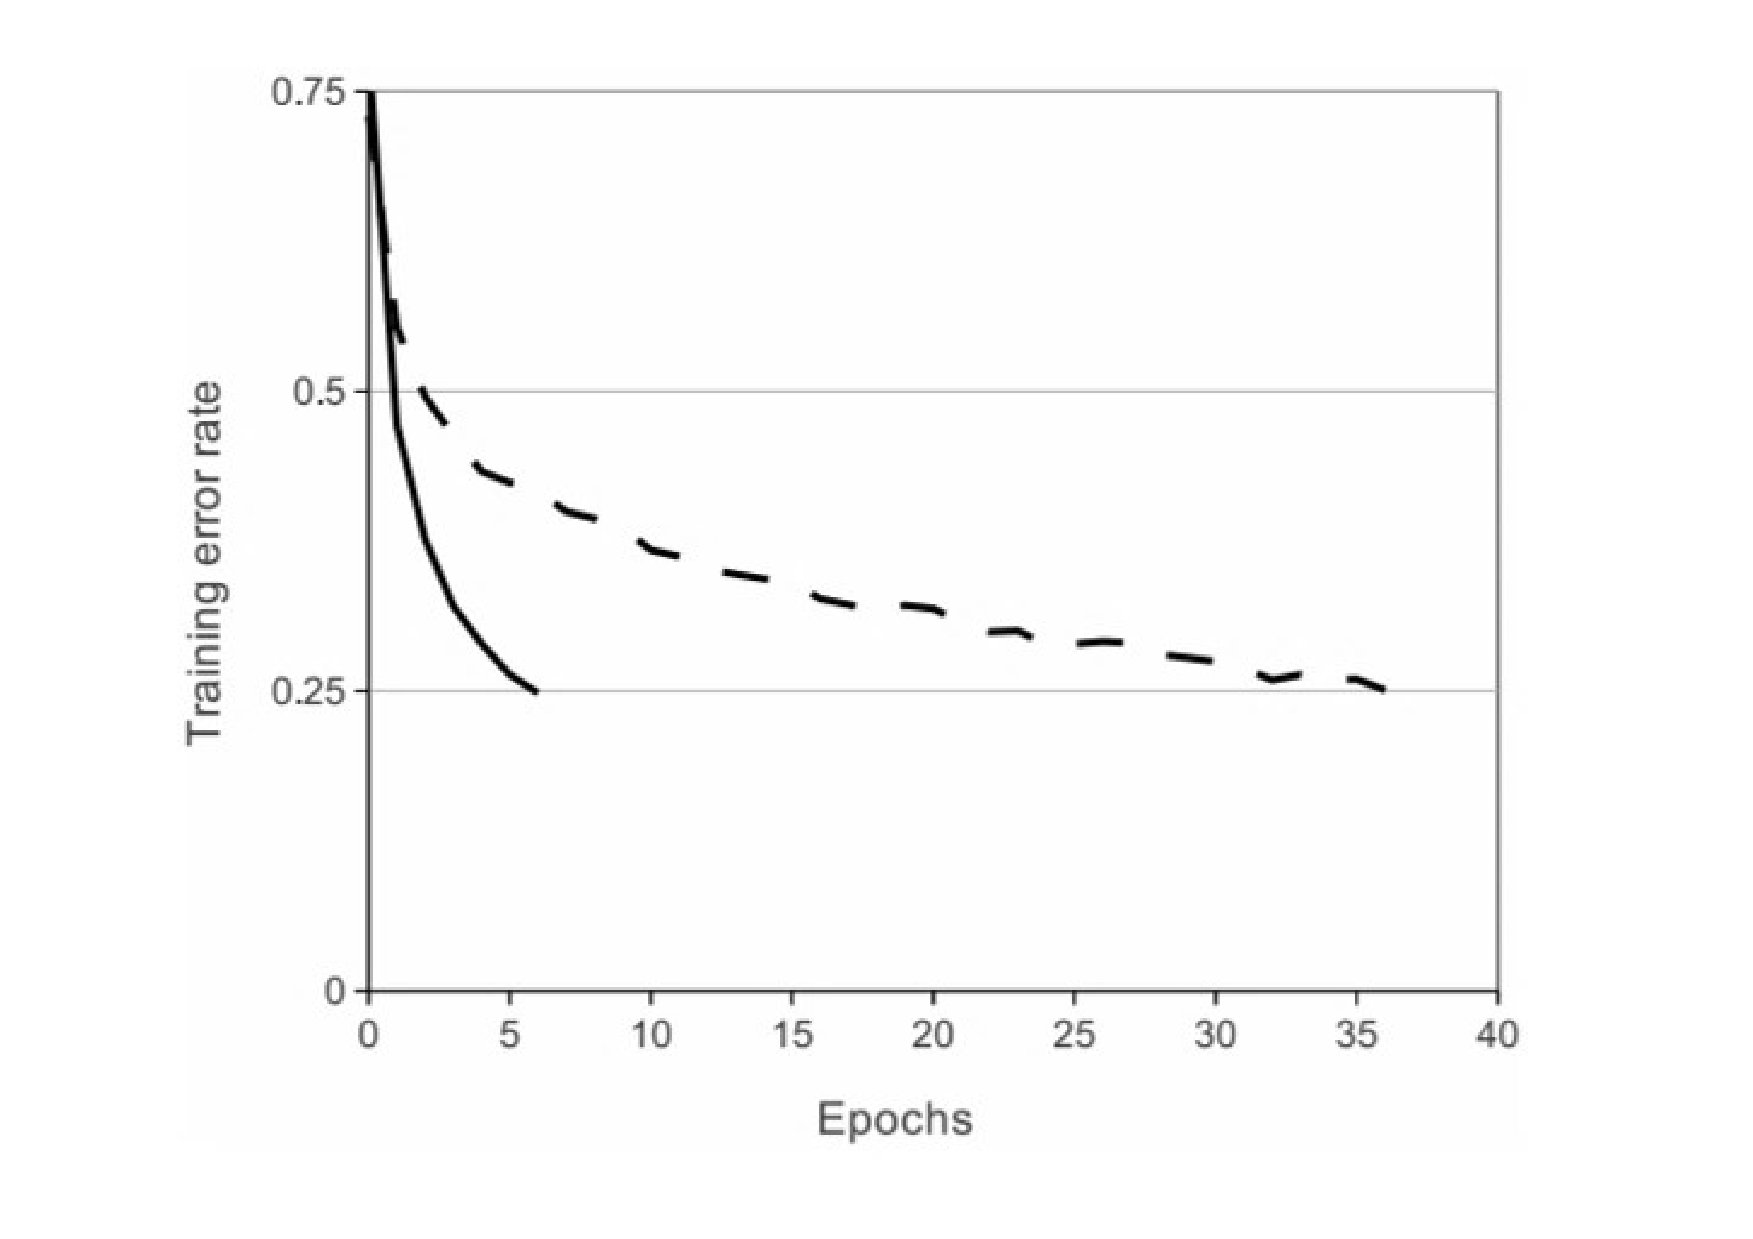
\includegraphics{1.pdf}}
  \caption{使用ReLU的四层卷积神经网络(实线)在CIFAR-10数据集上达到25\%的训练误差比使用tanh神经元的等价网络(虚线)快六倍。为了使训练尽可能快,每个网络的学习率是独立选取的。没有采用任何类型的正则化。这里演示的效果因网络结构的不同而不同,但带ReLU的网络学习始终比带饱和神经元的同等网络快好几倍。}
  \label{fig:fig1}
\end{figure}

\subsection{多GPU并行训练}
单个的GTX580 GPU只有3GB内存,这限制了可以在其上训练的网络的最大规模。事实证明,120万个训练样本足以训练那些因规模太大而不适合使用一个GPU训练的网络。因此,我们将网络分布在两个GPU上。目前的GPU很适合于跨GPU并行化操作,因为它们能够直接读写对方的内存,而无需通过主机内存。我们采用的这种并行模式主要是将一半的网络内核(或神经元)放在每个GPU上,然后再采用一个小技巧:将GPU通信限制在某些特定的层上。这意味着,比如,第三层的内核从所有的第二层内核映射(kernel map)中获得输入,但是,第四层的内核只从和自己在同一个GPU上的第三层内核中获得输入。选择连接模式对于交叉验证是一个不小的问题,但这使得我们能够精确调整通信量,直到它的计算量的达到可接受的程度。\\

由此产生的结构有点类似于Ciresan等人提出的“柱状”CNN的结构[5],不同之处在于我们的纵列不是独立的(见图2)。与一个GPU上训练的每个卷积层只有一半的内核数量的网络相比,该方案分别将我们的top-1和top-5错误率分别降低了1.7%和1.2%。双GPU结构网络比单GPU网络$\footnote{实际上单GPU网络与双GPU网络在最后的卷积层有着相同数量的核。这是因为大多数网络的参数在第一个全连接层,这需要上一个卷积层作为输入。所以,为了使两个网络有数目大致相同的参数,我们不把最后一个卷积层大小减半(也不把它后面跟随的全连接层减半)。因此,这种比较关系更偏向有利于单GPU网络,因为它比双GPU网络的“一半大小”要大}$所需的训练时间要稍微少一些。\\
	

\subsection{局部响应归一化}
ReLU具有让人满意的特性,它们无需对输入数据进行归一化(归一化的作用是来防止它们饱和)。如果至少一些训练样本对ReLU产生了正输入,那么学习将发生在那个神经元上。然而,我们仍然发现接下来的局部响应归一化有助于泛化。用$a_{x,y}^{i}$来表示在点$(x,y)$处通过先应用核$i$计算,然后再应用ReLU非线性计算出来的神经元激活度,响应归一化活性$b_{x,y}^{i}$由下面的式子给出
$$
b_{x,y}^{i}=a_{x,y}^{i}/\left ( k+\alpha \sum _{j=max(0,i-n/2)}^{min(N-1,i+n/2)}(a_{x,y}^{j})^{2} \right )^{\beta }
$$
求和运算在n个“毗邻的”核映射的同一位置上执行,N是本层的卷积核数目。核映射的顺序是任意的,这在训练开始前就确定了。响应归一化的顺序实现的是一种侧抑制形式,其灵感来源于真实神经元中的情况,这使得在使用不同核计算神经元输出的过程中创造了对大激活度的竞争。常量$k$,$n$,$\alpha$,$\beta$都是超参数,它们的值由验证集确定;我们设定$k=2$,$n=5$,$\alpha=10^{-4}$,$\beta=0.75$。我们在特定的层使用的ReLU非线性激活函数之后应用了这种归一化(请看3.5小节)。\\

该方案与Jarrett等人的局部对比度归一化方案具有一些相似之处[11],但是我们更正确的名称应该是“亮度归一化”,因为我们不减去平均活跃度。响应归一化将我们的top-1与top-5误差率分别减少了1.4\%与1.2\%。我们也验证了该方案在CIFAR-10数据集上的有效性:四层CNN不带归一化时的测试误差率是13\%,带归一化时是11\%$\footnote{由于篇幅有限,我们无法在这里十分详细的描述神经网络,更详细的参见代码以及代码当中的超参数,在这个网站你可以找到 http://code.google.com/p/cuda-convnet/.}$。

\subsection{重叠池化}
CNN中的池化层总结了同一核映射上相邻组神经元的输出。一般来说,相邻池化单元总结的邻近关系是不重叠的(例如[17,11,4])。更确切的说,池化层可看作由池化单元网格组成,网格间距为s个像素,每个网格归纳池化单元中心位置$z\times z$大小的邻居。如果设置$s=z$,我们会得到通常在CNN中采用的传统局部池化。如果设置$s < z$,我们会得到重叠池化。这就是我们网络中使用的方法,我们设置$s = 2$,$z = 3$。这个方案分别降低了top-1  0.4\%和top-5  0.3\%的错误率,与非重叠方案s = 2,z = 2相比,输出的维度是相等的。我们通常观察到在训练过程中有重叠池化的更加难以过拟合一些。

\begin{figure}[htbp]
  \centering
  \scalebox{0.6}{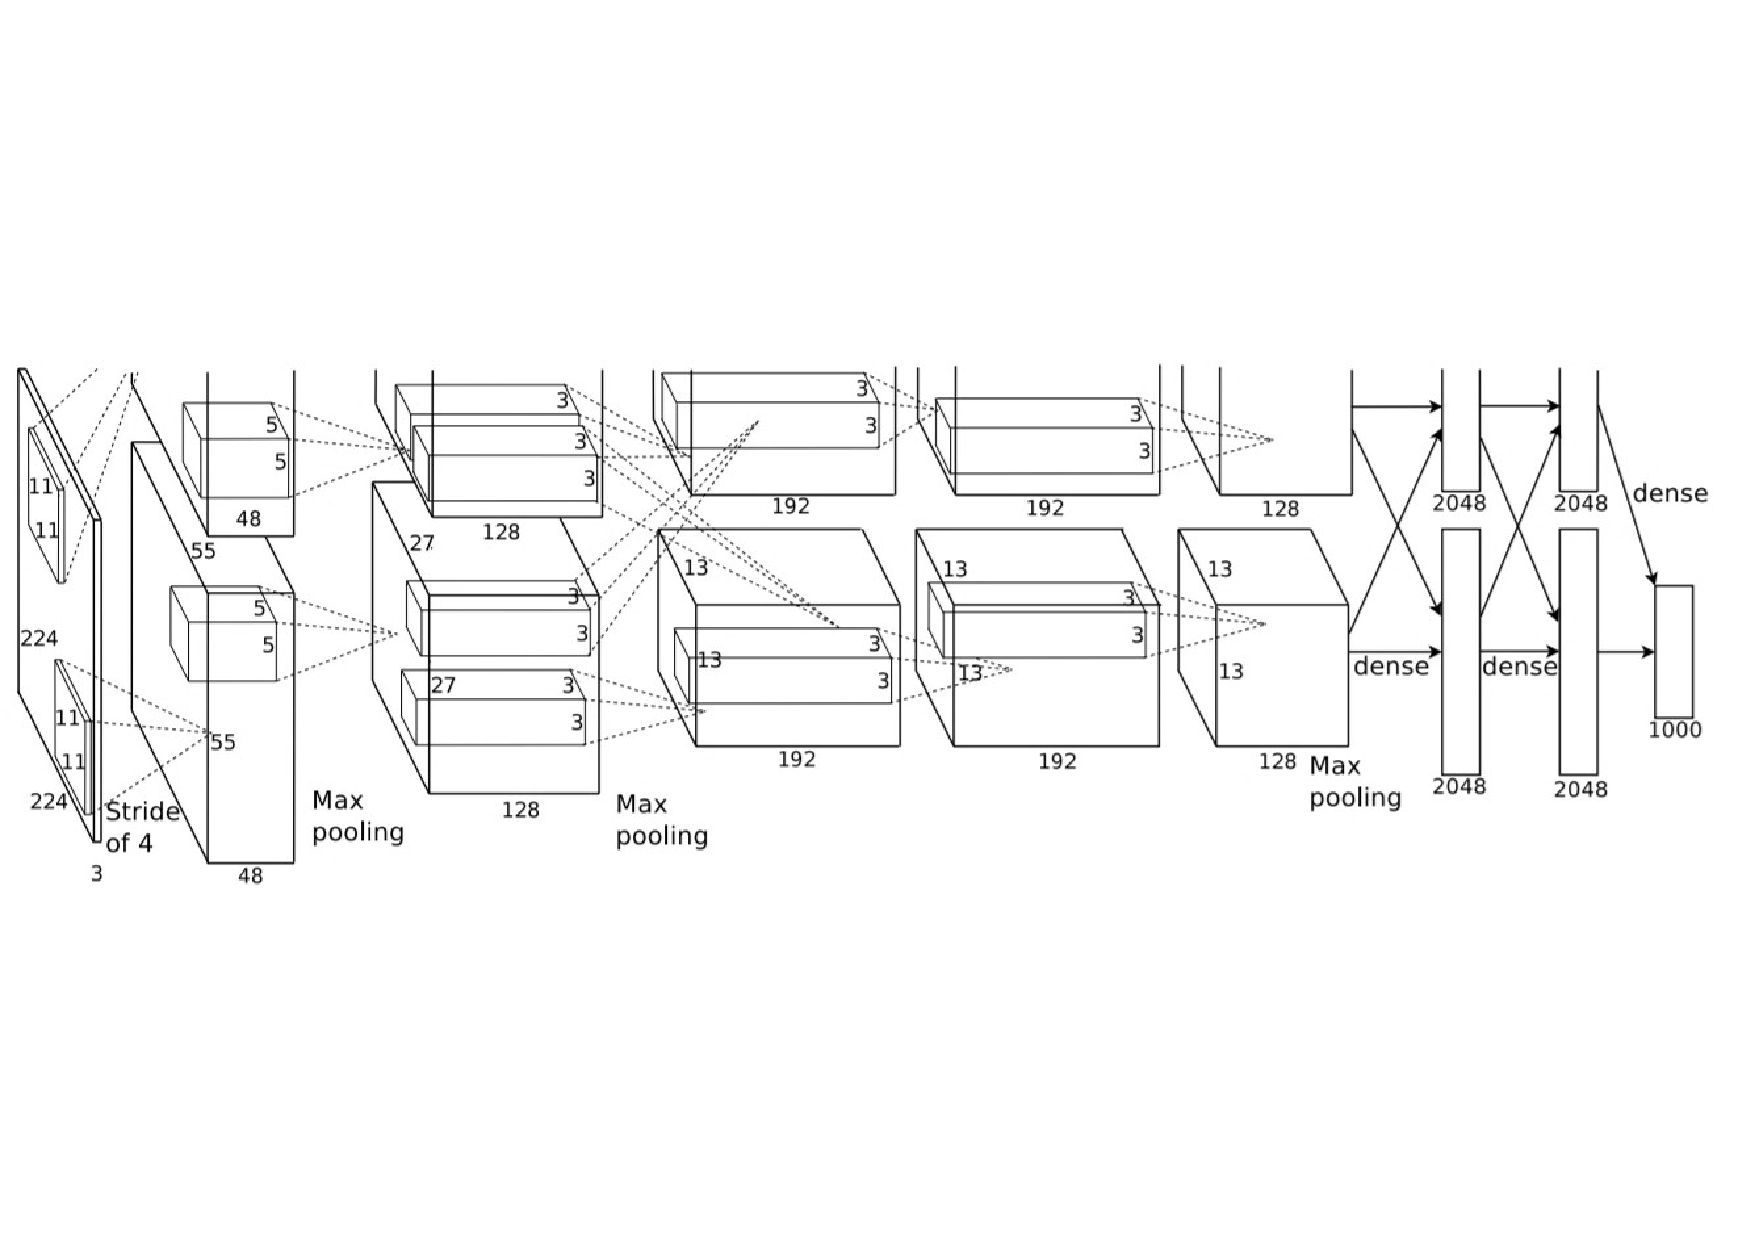
\includegraphics{2.pdf}}
  \caption{CNN体系结构示意图,明确显示了两个GPU之间的职责划分。一个GPU运行图中顶部的层次部分,而另一个GPU运行图中底部的层次部分。GPU之间仅在某些层互相通信。该网络的输入是150,528维的,且该网络剩下各层的神经元数分别为253,440–186,624–64,896–64,896–43,264–4096–4096–1000。}
  \label{fig:fig2}
\end{figure}

\subsection{总体结构}
现在,我们已经准备好描述我们CNN的总体结构。如图二所示,该网络包括了八个带权层;前五层是卷积层,剩下三层是全连接层。最后一个全连接层的输出被送到一个1000维的softmax层,softmax会产生一个覆盖1000类标签的分布。我们的网络使得多分类的Logistic回归目标最大化,这相当于最大化了预测分布下训练样本中正确标签的对数概率平均值。\\

第2,4,5卷积层的核只与位于同一GPU上的前一层的核映射相连接(看图2)。第3卷积层的核与第2层的所有核映射相连。全连接层的神经元与前一层的所有神经元相连。第1,2卷积层之后是响应归一化层。3.4节中描述的那种最大Pooling层,跟在响应归一化层以及第五个卷积层之后。ReLU非线性应用于每个卷积层及全连接层的输出。\\

第1卷积层使用96个大小为$11\times11\times3$,步长为4个像素(这是同一核映射中邻近神经元的感受野中心之间的距离)的核,来对大小为$224\times224\times3$的输入图像进行滤波。第2层卷积层使用第1层卷积层的输出(响应归一化和池化过的)作为输入,并使用了256个大小为$5\times5\times48$的核进行滤波。第3,4,5层卷积层互相连接,中间没有接入池化层或者归一化层。第3层有384个大小为$3\times3\times256$核与第2层卷积层的输出(响应归一化和池化过的)相连。第4层卷积层有384个大小为$3\times3\times192$的核,第5层有256个大小为$3\times3\times192$的核。全连接层每个都有4096个神经元。\\

\section{减少过拟合}
我们的神经网络结构有6000万参数。尽管ILSVRC的1000类使每个训练样本从图像到标签的映射上强加了10比特的约束,这依然不足以训练这么多的参数而不造成过拟合。接下来,我们会描述减少过拟合的两种主要方式。\\

\subsection{数据增强}
减少图像数据过拟合最简单最常用的方法,是使用标签-保留转换,人为地扩大数据集(例如,[25,4,5])。我们使用了两种独特的数据增强方式,这两种方式都可以从原始图像通过非常少的计算量产生变换的图像,因此变换图像不需要存储在硬盘上。在我们的实现中,变换图像通过CPU的Python代码生成,而此时GPU正在训练前一批图像。所以这种放大数据集的方式是很高效很节省计算资源的。\\

第一种数据增强的方式包括图像变换和水平翻转。我们通过从$256\times256$的图像上随机提取$224\times224$(译者注:此处应是227$\times$227)的图像块(及其水平镜像)的方法来实现,并在这些提取的图像$\footnote{这就是在图2中输入为224×224×3(译者注:此处应是227$\times$227$\times$3)的原因.}$上对我们的神经网络进行了训练。这通过一个2048因子增大了我们的训练集,尽管最终的训练样本是高度相关的。如果没有这个方案,我们的网络会出现严重的过拟合,这会迫使我们使用更小的网络。在测试时,网络会抽取五个$224\times224$(译者注:此处应是227$\times$227)的图像块(四个角上的图像块和中心的图像块)以及他们的水平翻转(总共是个图像块)进行预测,然后将softmax层对这十个图像块做出的预测取平均。\\

第二种放大数据集的方法是改变训练图像的RGB通道的强度。具体地,我们在整个ImageNet训练集上对RGB像素进行了PCA(主成分分析)。对于每张训练图像,我们通过均值为0,方差为0.1的高斯分布产生一个随机值a,然后通过向图像中加入更大比例的相应的本征值的a倍,把其主成分翻倍。因此,对于每个RGB像素$I_{xy}=\begin{bmatrix}
I_{xy}^{R} & I_{xy}^{G} & I_{xy}^{B} 
\end{bmatrix}^{T}$,我们加入的值如下:\\
$$
\begin{bmatrix}
P_{1} & P_{2} & P_{3}
\end{bmatrix}
\begin{bmatrix}
\alpha _{1}\lambda _{1} & \alpha_{2}\lambda _{2} & \alpha _{3}\lambda _{3}
\end{bmatrix}^{T}
$$

其中,$P_{i}$和$\lambda _{i}$分别是RGB像素值$3\times3$协方差矩阵的第$i$个特征向量和特征值,$\alpha ^{i}$是前面提到的随机变量。对于某个训练图像的所有像素,每个$\alpha ^{i}$只获取一次,直到图像进行下一次训练时才重新获取。这个方案近似抓住了自然图像的一个重要特性,即光照的颜色和强度发生变化时,目标是不变的。这一方法把top-1错误降低了1\%。


\subsection{随机失活}
将许多不同模型的预测结合起来是降低测试误差[1, 3]的一个非常成功的方法,但这种方法对于本来就需要花费几天去训练的大型神经网络来说,代价太过高昂。然而,有一个非常有效的模型结合方法,它只花费两倍于单模型的训练成本。这种最新引入的技术,叫做“dropout”[10],它以0.5的概率将每个隐层神经元的输出设置为0。这些“失活的”神经元既不在参与前向传播,也不再参与反向传播。所以每次输入时,神经网络会采用一个不同的架构,但是这所有的架构共享权重。这种技术降低了神经元之间复杂的互适应关系,因为一个神经元不能再依赖特定的神经元而存在了。因此,神经元被迫学习更具鲁棒性的特征,这些特征在结合其他神经元的一些不同随机子集时有用。在测试时,我们将所有的神经元的输出都乘以0.5,对指数级的许多失活网络的预测分布进行几何平均,这是一种合理的近似方法。\\

我们在图二的前两个全连接层中使用了dropout。如果没有dropout,我们的网络将会严重的过拟合。Dropout使得收敛所需要的迭代次数翻了一倍。

\section{学习细节}
我们使用随机梯度下降来训练我们的模型,样本的batch size是128,momentum是0.9,权重衰减为0.0005。我们发现这里少量的权重衰减对于模型的学习是很重要的。换句话说,权重衰减在这里不仅仅是一个正则化项:它减少了模型的训练误差。对于权重w的更新规则为\\
$$
v_{i+1} := 0.9 \cdot v_{i} - 0.0005\cdot \epsilon \cdot w_{i}-\epsilon \cdot \left \langle \frac{\partial L}{\partial w}\mid _{w_{i}} \right \rangle _{D_{i}}
$$

$$
w_{i+1}:=w_{i}+v_{i+1}
$$


我们使用均值为0,标准差为0.01的高斯分布对每一层的权重进行初始化。我们用常数1初始化了第二、四、五卷积层和全连接层的神经元的偏置项。这个初始化通过为ReLU提供正输入加速了学习的早期阶段。我们用常数0初始化了其余层神经元的偏置项。\\

我们对所有层都使用了相同的学习率,这是我们在训练过程中手动调整的。我们遵循的一些原则是:当验证误差率在当前学习率下不再提高时,就将学习率除以10。学习率初始化为0.01,在训练停止之前降低了三次。我们训练该网络时大致将这120万张图像的训练集循环了90次,在两个NVIDIA GTX 580 3GB GPU上花了五到六天。\\



\section{结果}
我们将ILSVRC-2010测试集上的结果概括为表1。我们的网络实现了top-1测试集误差率为37.5\%,top-5测试集误差率为17.0\%$\footnote{如第4.1节所述,没有对10个patches进行求平均,则预测的错误率分别为39.0%和18.3%。}$。在ILSVRC-2010竞赛中的最佳结果是47.1\%与28.2\%,,它们的方法是用不同特征训练六个sparse-coding模型,对这些模型产生的预测求平均值。从那之后公布的最好结果是45.7\%和25.7\%,它们的方法是从两类密集采样的特征中计算出费舍尔向量(FV),用费舍尔向量训练两个分类器,再对这两个分类器的预测求平均值[24]。\\
\begin{table}
  \centering
  \begin{tabular}{lll}
    \toprule
    \textbf{Model}     & \textbf{Top-1}      &\textbf{Top-5}  \\
    \midrule
    \emph{Sparse coding [2] } & \emph{47.1\%}   & \emph{28.2\%}      \\
    \emph{SIFT + FVs [24]}      & \emph{45.7\%} & \emph{20.7\%}     \\
    CNN     & \textbf{37.5\%}       & \textbf{17.0\%}  \\
    \bottomrule
  \end{tabular}
  \caption{ILSVRC-2010测试集上的结果比较。斜体字是他人取得的最好结果。}
  \label{tab:table}
\end{table}

我们也使用我们的模型参加了ILSVRC-2012竞赛,并在表2中写出了结果。因为ILSVRC-2012的测试集标签是不对外公开的,我们无法报告我们尝试的所有模型的测试误差率。在这段的剩余部分,我们将验证误差率和测试误差率互换,因为根据我们的经验,它们之间不会相差超过0.1\%(见表2)。本文描述的CNN取得了18.2\%的top-5误差率。五个类似的CNN预测的平均误差率为16.4\%。为了对ImageNet 在2011秋季发布的整个数据集(1500万张图片,22000个类别)进行分类,我们在最后的池化层之后增加了一个额外的第六层卷积层,训练了一个新的CNN,然后对它进行“fine-tuning”,最后在ILSVRC-2012上取得了16.6\%的错误率。对在ImageNet 2011秋季发布的整个数据集上预训练的两个CNN和前面提到的五个CNN的预测进行平均得到了15.3\%的错误率。第二名的成绩是26.2\%的误差率,它的方法是从不同类密集采样的特征中计算FV,用FV训练几个分类器,再对这几个分类器的预测求平均值[7]。\\
\begin{table}
  \centering
  \begin{tabular}{llll}
    \toprule
    \textbf{Model} & \textbf{Top-1(val)} &\textbf{Top-5(val)} & \textbf{Top-5(test)}\\
    \midrule
    \emph{SIFT + FVs [7]} &  —   &   —  &  \emph{26.2\%} \\
    1CNN     & 40.7\% & 18.2\%   &       —           \\
    5CNNs    & 38.1\% & 16.4\%   &\textbf{16.4\%}  \\
	1CNN*    & 39.0\% & 16.6\%   &   —  \\
	7CNNs*   & 36.7\% & 15.4\%   &\textbf{15.3\%}\\
    \bottomrule
  \end{tabular}
  \caption{ILSVRC-2010测试集上的结果比较。斜体字是他人取得的最好结果。}
  \label{tab:table}
\end{table}


最后,我们也报告了我们在ImageNet 2009秋季数据集上的误差率,ImageNet 2009秋季数据集有10,184个类,890万图像。在这个数据集上,按照惯例,我们用一半的图像来训练,一半的图像来测试。由于没有明确的测试集,我们的划分必然不同于以前作者的数据集划分,但这不会明显的影响到结果。我们在这个数据集上的的top-1和top-5错误率是67.4\%和40.9\%,使用的是上面描述的在最后的池化层之后有一个额外的第6卷积层网络。该数据集上公布的最佳结果是78.1\%和60.9\%[19]。\\



\begin{figure}[h]
  \centering
  \scalebox{0.4}{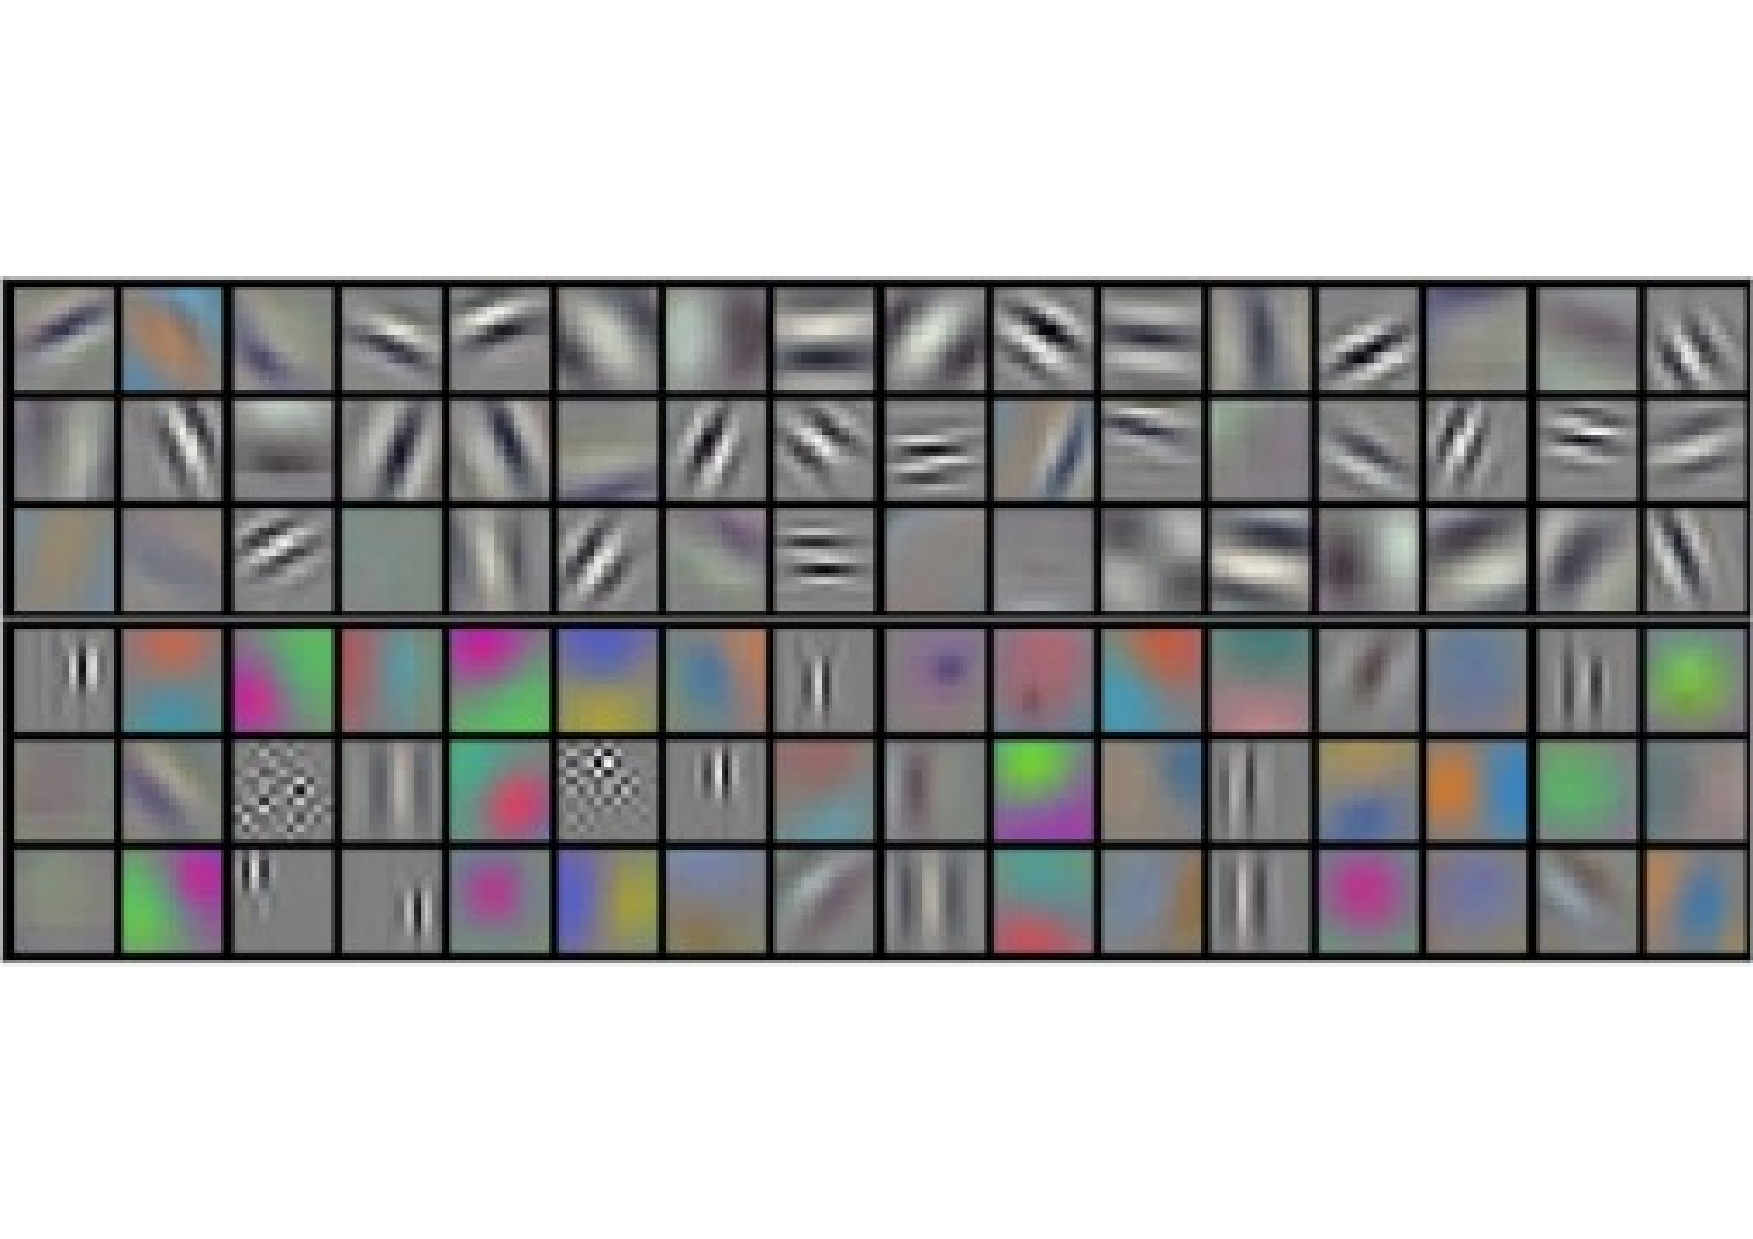
\includegraphics{3.pdf}}
  \caption{第一卷积层在224×224×3(译者注:应该是227×227×3)的输入图像上学习到的大小为11×11×3的96个卷积核。上面的48个核是在GPU 1上学习到的而下面的48个卷积核是在GPU 2上学习到的。更多细节请看6.1小节。}
  \label{fig:fig3}
\end{figure}

\subsection{定性评价}
图三显示了网络的两个数据连接层学习到的卷积核。该网络已经学习到了各种各样的频率与方向选择核,以及各种颜色点。注意两个GPU显示出的特性,3.5节中描述了一个结果是限制连接。GPU1上的核大部分颜色不明确,而GPU2上的核大多数颜色明确。这种特性在每一次运行中都会出现,且独立于所有特定的随机权重初始化(以GPU的重新编数为模)。\\ 

在图四的左边部分,通过计算该网络在八个测试图像上的top-5预测,我们可以定性的评估它到底学习到了什么。注意到即使是偏离中心的物体,比如左上角的一个小虫,也可以被网络识别到。大多数的top-5标签似乎是合理的。例如,对于美洲豹来说,只有其他类型的猫被认为是看似合理的标签。在某些情况下(铁栅、樱桃),对于图片意图的焦点存在歧义。\\

\begin{figure}[h]
  \centering
  \scalebox{0.6}{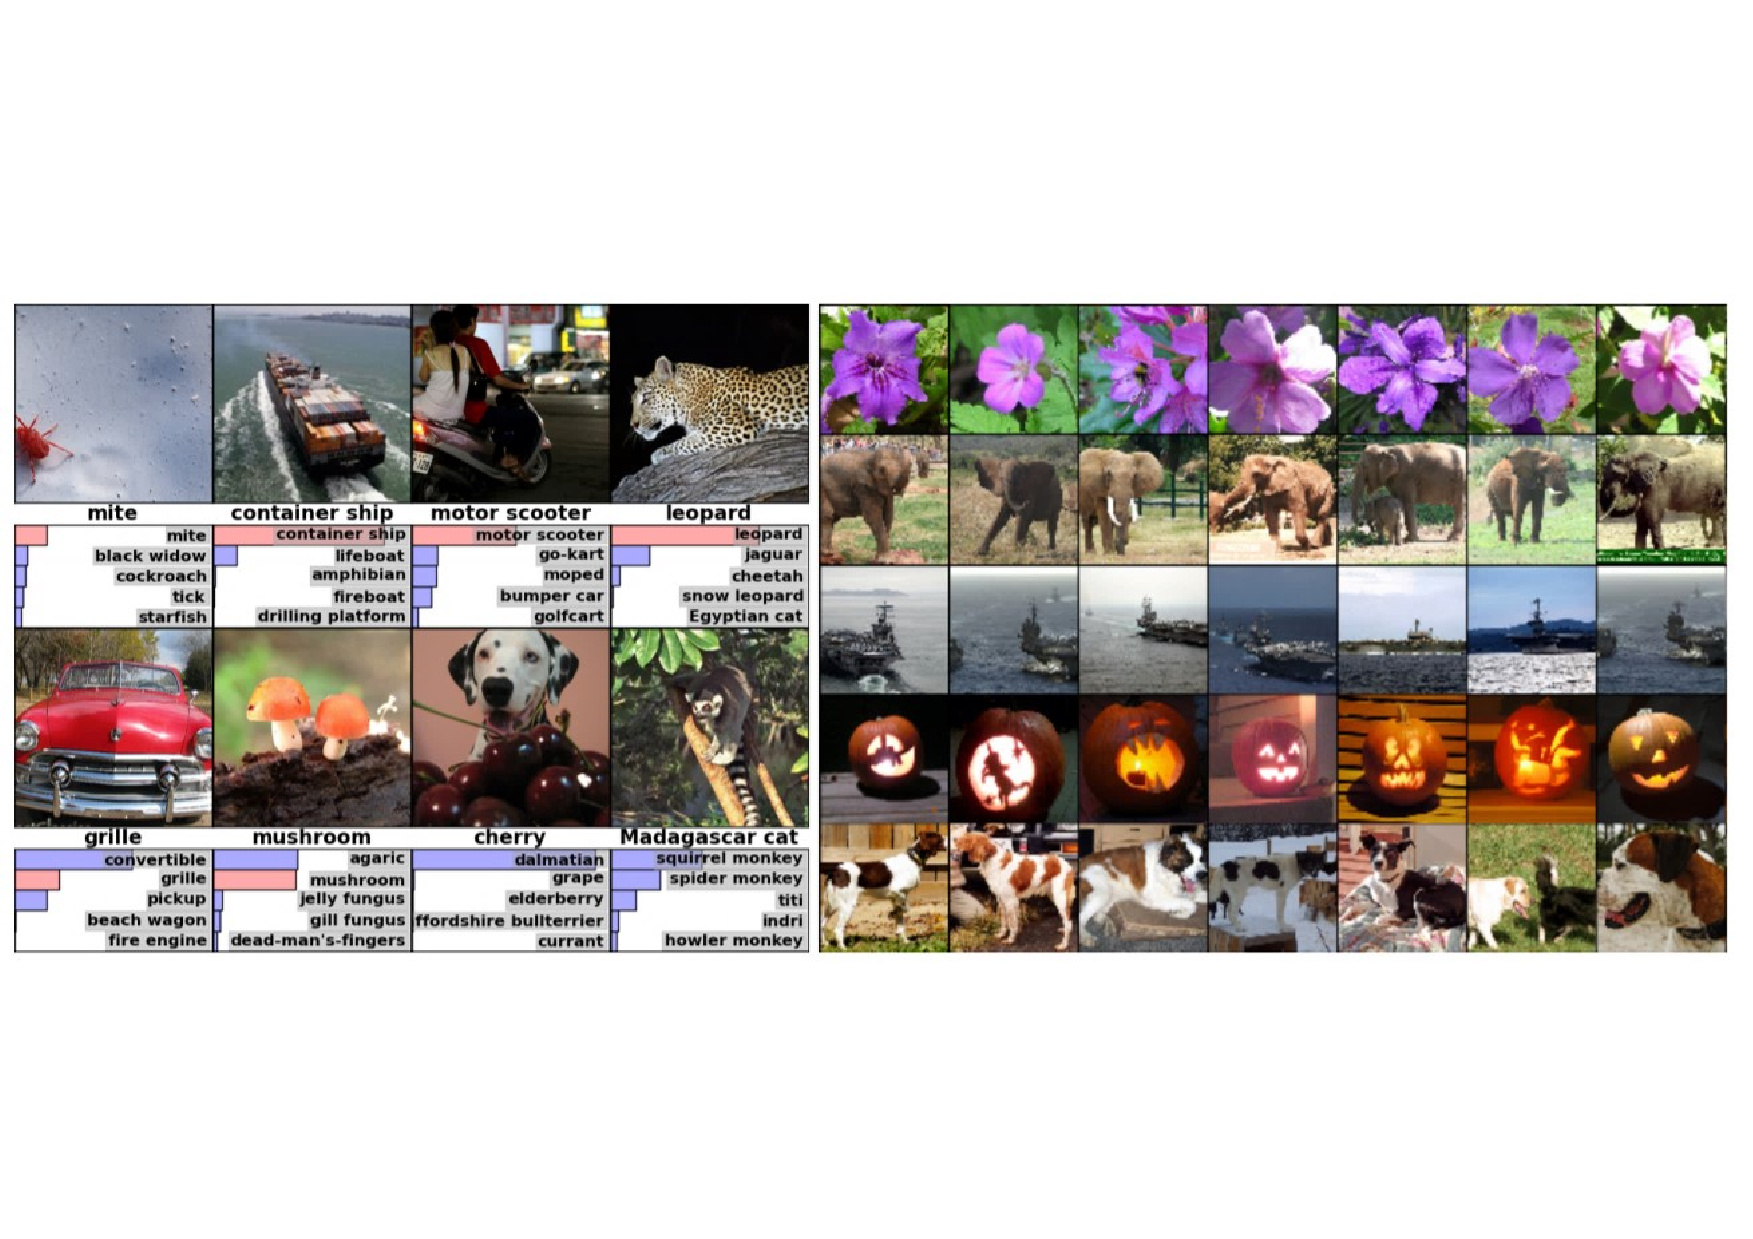
\includegraphics{4.pdf}}
  \caption{(左)8张ILSVRC-2010测试图像和我们的模型认为最可能的5个标签。每张图像的下面是它的正确标签,正确标签的概率用红条表示(如果正确标签在前五当中)。(右)第一列是5张ILSVRC-2010测试图像。剩下的列展示了6张训练图像,这些图像的最后的隐藏层的特征向量与测试图像的特征向量有最小的欧氏距离。}
  \label{fig:fig4}
\end{figure}

另外一个探索网络可视化知识的方法是考虑最后4096维隐藏层在图像上得到的特征激活。如果两幅图像生产的特征激活向量之间有较小的欧氏距离,我们可以说,在神经网络更高级别上认为它们是相似的。图四展示了测试集中的五个图像,以及训练集中根据这一标准与其中每一个最相似的六个图像。注意,在像素级别,检索到的训练图像一般不会接近第一列中的查询图像。例如,检索到的狗和大象表现出各种各样的姿势。我们会在补充材料里给出更多测试图像的结果。\\

通过使用两个4096维实值向量间的欧氏距离来计算相似性是效率低下的,但它可以通过训练一个自编码器将这些向量压缩为短的二进制代码来变得高效。这应该会产生一个比将自编码器直接应用到原始图像上好得多的图像检索方法[14],它不利用图像标签,因此会趋向于检索与要检索的图像具有相似边缘模式的图像,而不论它们在语义上是否相似。\\



\section{讨论}
我们的结果表明大型深度卷积神经网络在一个非常具有挑战性的数据集上使用纯粹的监督学习,能够达到破纪录的效果。值得注意的是,如果有一个卷积层被移除,我们的网络性能就会降低。例如,除去任何中间层都将导致网络的top-1性能有2\%的损失。所以深度对于实现我们的结果真的是很重要的。\\

为了简化我们的实验,我们没有使用任何无监督的预训练,尽管我们预计它会有所帮助,特别是在如果我们能获得足够的计算能力来显著增加网络的大小而标注的数据量没有对应增加的情况下。因此,到目前为止,我们的结果已经提高了,因为我们的网络更大、训练时间更长,但为了匹配人类视觉系统的infero-temporal路径,我们仍然有更高的数量级要去达到。最终我们想在视频序列上使用非常大型的深度卷积网络,视频序列的时序结构会提供非常有帮助的信息,这些信息在静态图像上是缺失的或极不明显。




\bibliographystyle{unsrt}  
%\bibliography{references} 
%%% Remove comment to use the external .bib file (using bibtex).
%%% and comment out the ``thebibliography'' section.

%%% Comment out this section when you \bibliography{references} is enabled.
\begin{thebibliography}{1}

\bibitem{1}
R.M.BellandY.Koren.
\newblock Lessons from the netflix prize challenge.
\newblock {\em ACM SIGKDD Explorations Newsletter},9(2):75–79, 2007. 

\bibitem{2}
A. Berg, J. Deng, and L. Fei-Fei. 
\newblock Large scale visual recognition challenge 2010. 
\newblock www.imagenet.org/challenges. 2010. 

\bibitem{3}
L. Breiman. 
\newblock Random forests.
\newblock {\em Machine learning},45(1):5–32, 2001. 

\bibitem{4}
D. Cires¸an, U. Meier, and J. Schmidhuber.  
\newblock Multi-column deep neural networks for image classification. 
\newblock {\em Arxiv preprint arXiv:1202.2745},2012.

\bibitem{5}
D.C. Cires¸an, U. Meier, J. Masci, L.M. Gambardella, and J. Schmidhuber.   
\newblock High-performance neural networks for visual object classification. 
\newblock {\em Arxiv preprint arXiv:1102.0183},2011.

\bibitem{6}
J. Deng, W. Dong, R. Socher, L.-J. Li, K. Li, and L. Fei-Fei. 
\newblock ImageNet: A Large-Scale Hierarchical Image Database.
\newblock {\em In CVPR09},2009.

\bibitem{7}
J. Deng, A. Berg, S. Satheesh, H. Su, A. Khosla, and L. Fei-Fei.  
\newblock ImageNet: A Large-Scale Hierarchical Image Database.
\newblock {\em ILSVRC-2012},2012.  URL http://www.image-net.org/challenges/LSVRC/2012/. 

\bibitem{8}
L. Fei-Fei, R. Fergus, and P. Perona. 
\newblock  Learning generative visual models from few training examples:  An incremental bayesian approach tested on 101 object categories. 
\newblock {\em Computer Vision and Image Understanding}, 106(1):59–70, 2007.

\bibitem{9}
G. Griffin, A. Holub, and P. Perona.
\newblock Caltech-256 object category dataset. 
\newblock Technical Report 7694, California Institute of Technology, 2007. URL http://authors.library.caltech.edu/7694.

\bibitem{10}
G.E. Hinton, N. Srivastava, A. Krizhevsky, I. Sutskever, and R.R. Salakhutdinov.  
\newblock  Improving neural networks by preventing co-adaptation of feature detectors. 
\newblock {\em arXiv preprint arXiv:1207.0580},2012.

\bibitem{11}
K. Jarrett, K. Kavukcuoglu, M. A. Ranzato, and Y. LeCun. 
\newblock What is the best multi-stage architecture for object recognition?
\newblock In {\em International Conference on Computer Vision},pages 2146–2153. IEEE, 2009. 

\bibitem{12}
A. Krizhevsky. 
\newblock Learning multiple layers of features from tiny images. 
\newblock Master’s thesis, Department of Computer Science, University of Toronto, 2009. 

\bibitem{13}
A. Krizhevsky.  
\newblock Convolutional deep belief networks on cifar-10. 
\newblock {\em Unpublished manuscript},2010.

\bibitem{14}
A. Krizhevsky and G.E. Hinton.  
\newblock Using very deep autoencoders for content-based image retrieval. 
\newblock In {\em ESANN},2011.

\bibitem{15}
Y. Le Cun, B. Boser, J.S. Denker, D. Henderson, R.E. Howard, W. Hubbard, L.D. Jackel, et al.  
\newblock Hand-written digit recognition with a back-propagation network. 
\newblock In {\em Advances in neural information processing systems},1990.

\bibitem{16}
Y. LeCun, F.J. Huang, and L. Bottou.  
\newblock Learning methods for generic object recognition with invariance to pose and lighting.
\newblock In {\em   Computer Vision and Pattern Recognition, 2004. CVPR 2004. Proceedings of the 2004 IEEE Computer Society Conference on},volume 2, pages II–97. IEEE, 2004.

\bibitem{17}
Y. LeCun, K. Kavukcuoglu, and C. Farabet. 
\newblock Convolutional networks and applications in vision. 
\newblock In {\em Circuits and Systems (ISCAS), Proceedings of 2010 IEEE International Symposium on}, pages 253–256. IEEE, 2010. 
\bibitem{18}
H. Lee, R. Grosse, R. Ranganath, and A.Y. Ng.  
\newblock  Convolutional deep belief networks for scalable unsupervised learning of hierarchical representations.  
\newblock In {\em Proceedings of the 26th Annual International Conference on Machine Learning},pages 609–616. ACM, 2009. 

\bibitem{19}
T. Mensink, J. Verbeek, F. Perronnin, and G. Csurka.   
\newblock Metric Learning for Large Scale Image Classification: Generalizing to New Classes at Near-Zero Cost. 
\newblock In {\em  ECCV - European Conference on Computer Vision, Florence, Italy},October 2012.

\bibitem{20}
V. Nair and G. E. Hinton. 
\newblock Rectified linear units improve restricted boltzmann machines.  
\newblock In {\em Proc. 27th International Conference on Machine Learning},2010.

\bibitem{21}
N. Pinto, D.D. Cox, and J.J. DiCarlo.  
\newblock Why is real-world visual object recognition hard?  
\newblock {\em PLoS computational biology},4(1):e27, 2008. 

\bibitem{22}
N. Pinto, D. Doukhan, J.J. DiCarlo, and D.D. Cox.  
\newblock A high-throughput screening approach to discovering good forms of biologically inspired visual representation. 
\newblock {\em  PLoS computational biology},5(11):e1000579, 2009. 

\bibitem{23}
B.C. Russell, A. Torralba, K.P. Murphy, and W.T. Freeman.  
\newblock Labelme: a database and web-based tool for image annotation.
\newblock {\em  International journal of computer vision},77(1):157–173, 2008.

\bibitem{24}
J.SánchezandF.Perronnin.  
\newblock High-dimensional signature compression for large-scale image classification.
\newblock In {\em Computer Vision and Pattern Recognition(CVPR),2011 IEEE Conference on},pages1665–1672.IEEE, 2011. 
 
\bibitem{25}
P.Y. Simard, D. Steinkraus, and J.C. Platt.   
\newblock Best practices for convolutional neural networks applied to visualdocumentanalysis. 
\newblock In {\em Proceedings of the Seventh International Conference on Document Analysis and Recognition},volume 2, pages 958–962, 2003.

\bibitem{26}
S.C.Turaga,J.F.Murray,V.Jain,F.Roth,M.Helmstaedter,K.Briggman,W.Denk,andH.S.Seung.  
\newblock  Convolutional networks can learn to generate affinity graphs for image segmentation. 
\newblock {\em Neural Computation},22(2):511–538, 2010.



\end{thebibliography}

\end{CJK*}
\end{document}
